\documentclass[12pt]{article}
\usepackage{amsfonts,amssymb,float,amsmath}
\usepackage{algorithmic}
\usepackage{graphicx, siunintx}
\usepackage{textcomp}
\usepackage{xcolor}
\usepackage{txfonts}
\usepackage{multicol}
\usepackage{listings}
\usepackage{enumitem}
\usepackage{mathtools}
\usepackage{gensymb}
\usepackage{comment}
\usepackage[breaklinks=true]{hyperref}
\usepackage{tkz-euclide} 
\usepackage{listings}
\usepackage{gvv}                       
\usepackage{gvv-book}
%\def\inputGnumericTable{}                             
\usepackage{color}                                            
\usepackage{array}                                            
\usepackage{longtable}                                       
\usepackage{calc}                                             
\usepackage{multirow}                                         
\usepackage{hhline}                                           
\usepackage{ifthen}                                           
\usepackage{lscape}
\newcommand{\BEQA}{\begin{eqnarray}}
\newcommand{\EEQA}{\end{eqnarray}}
%\newcommand{\define}{\stackrel{\triangle}{=}}
\theoremstyle{remark}
\newtheorem{rem}{Remark}
\parindent 0px
\pagenumbering{gobble}
\begin{document}
\title{\vspace{-5cm}Gate paper 2023-XH}
\author{Ayush Sunil Labhade}
\date{AI25Btech11002}
\maketitle

\begin{flushright}Humanities and Social Sciences – Philosophy (XH-C4)\end{flushright}
\begin{flushleft}General Aptitude \textbf{\brak{GA}} \\[5pt]
\textbf{\item Q.1 – Q.5 Carry ONE mark Each}\end{flushleft}
\begin{enumerate}
%Q.1
\item Rafi told Mary, “I am thinking of watching a film this weekend.”
The following reports the above statement in indirect speech: 
Rafi told Mary that he \_\_\_\_\_\_\_ of watching a film that weekend.
\begin{enumerate} 
    \begin{multicols}{2}
        \item thought
        \item is thinking
        \item am thinking
        \item was thinking
    \end{multicols} 
\end{enumerate}
\hfill\brak{GATE \ XH \ 2023}
%Q.2
\item Permit : \_\_\_\_\_\_\_ : : Enforce : Relax 
\brak{By word meaning}
\begin{enumerate} 
    \begin{multicols}{4}
        \item Allow
        \item Forbid
        \item License
        \item Reinforce
    \end{multicols} 
\end{enumerate}
\hfill\brak{GATE \ XH \ 2023}
%Q.3
\item Given a fair six-faced dice where the faces are labelled ‘1’, ‘2’, ‘3’, ‘4’, ‘5’, and ‘6’, 
what is the probability of getting a ‘1’ on the first roll of the dice and a ‘4’ on the 
second roll?
\begin{enumerate} 
    \begin{multicols}{4}
        \item $\frac{1}{36}$
        \item $\frac{1}{6}$
        \item $\frac{5}{6}$
        \item $\frac{1}{3}$
    \end{multicols} 
\end{enumerate}
\hfill\brak{GATE \ XH \ 2023}
%Q.4
\item A recent survey shows that 65% of tobacco users were advised to stop consuming tobacco.
The survey also shows that 3 out of 10 tobacco users attempted to stop using tobacco.
Based only on the information in the above passage, which one of the following options can be logically inferred with certainty?
\begin{enumerate}
    \item A majority of tobacco users who were advised to stop consuming tobacco made an attempt to do so.
    \item A majority of tobacco users who were advised to stop consuming tobacco did not attempt to do so.
    \item Approximately 30% of tobacco users successfully stopped consuming tobacco.
    \item Approximately 65% of tobacco users successfully stopped consuming tobacco.
\end{enumerate}
\hfill\brak{GATE \ XH \ 2023}
%Q.5
\item How many triangles are present in the given figure?
\begin{figure}[H]
    \centering
    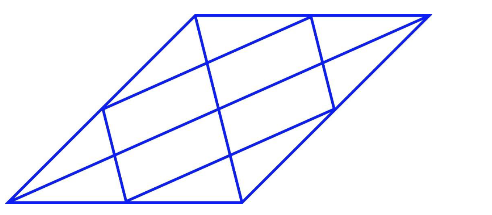
\includegraphics[width=0.5\textwidth]{Figs/Q5.png}
    \caption{}
    \label{fig:4.1}
\end{figure}
\begin{enumerate}
    \begin{multicols}{4}
        \item 12
        \item 16
        \item 20
        \item 24
    \end{multicols}
\end{enumerate}
\hfill\brak{GATE \ XH \ 2023}
\newpage
\textbf{Q.6 – Q.10 Carry TWO marks Each}
%Q.6
\item Students of all the departments of a college who have successfully completed the registration process are eligible to vote in the upcoming college elections. However, by the time the due date for registration was over, it was found that surprisingly none of the students from the Department of Human Sciences had completed the registration process. Based only on the information provided above, which one of the following sets of statement(s) can be logically inferred with certainty?
\begin{enumerate}
    \item[(i)] All those students who would not be eligible to vote in the college elections would certainly belong to the Department of Human Sciences.
    \item[(ii)] None of the students from departments other than Human Sciences failed to complete the registration process within the due time.
    \item[(iii)] All the eligible voters would certainly be students who are not from the Department of Human Sciences.
\end{enumerate}
\begin{enumerate}
    \begin{multicols}{4}
        \item (i) and (ii)
        \item (i) and (iii)
        \item only (i)
        \item only (iii)
    \end{multicols}
\end{enumerate}
\hfill\brak{GATE \ XH \ 2023}
%Q.7
\item Which one of the following options represents the given graph?
\begin{figure}[H]
    \centering
    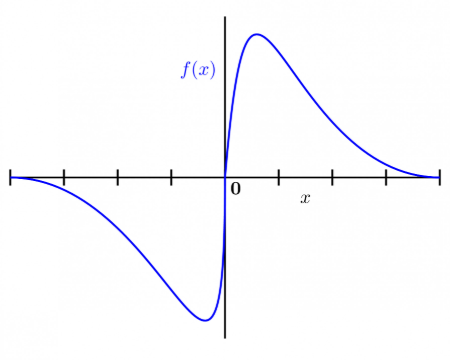
\includegraphics[width=0.6\textwidth]{Figs/Q7.png}
    \caption{}
    \label{fig:4.2}
\end{figure}
\begin{enumerate}
    \begin{multicols}{4}
        \item $f(x)=x^22^{-|x|}$ 
        \item $f(x)=x2^{-|x|}$
        \item $f(x)=|x|2^{-x}$ 
        \item $f(x)=x2^{-x}$
    \end{multicols}
\end{enumerate}
\hfill\brak{GATE \ XH \ 2023}
%Q.8
\item Which one of the options does NOT describe the passage below or follow from it?
We tend to think of cancer as a ‘modern’ illness because its metaphors are so modern. It is a disease of overproduction, of sudden growth, a growth that is unstoppable, tipped into the abyss of no control. Modern cell biology encourages us to imagine the cell as a molecular machine. Cancer is that machine unable to quench its initial command \brak{to grow} and thus transform into an indestructible, self-propelled automaton.
\sbrak{Adapted from \textit{The Emperor of All Maladies} by Siddhartha Mukherjee}
\begin{enumerate}
    \item It is a reflection of why cancer seems so modern to most of us.
    \item It tells us that modern cell biology uses and promotes metaphors of machinery.
    \item Modern cell biology encourages metaphors of machinery, and cancer is often imagined as a machine.
    \item Modern cell biology never uses figurative language, such as metaphors, to describe or explain anything.
\end{enumerate}
\hfill\brak{GATE \ XH \ 2023}
%Q.9
\item The digit in the unit’s place of the product $3^{999} \times 7^{1000}$ is \_\_\_\_\_\_\_.
\begin{enumerate}
    \begin{multicols}{4}
        \item 7
        \item 1
        \item 3
        \item 9
    \end{multicols}
\end{enumerate}
\hfill\brak{GATE \ XH \ 2023}
%Q.10
\item A square with sides of length 6 cm is given. The boundary of the shaded region is defined by two semi-circles whose diameters are the sides of the square, as shown. The area of the shaded region is \_\_\_\_\_\_\_ cm$^2$.
\begin{figure}[H]
    \centering
    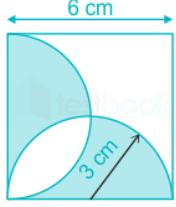
\includegraphics[width=0.3\textwidth]{Figs/Q10.png}
    \caption{}
    \label{fig:4.3}
\end{figure}
\begin{enumerate}
    \begin{multicols}{4}
        \item $6\pi$
        \item 18
        \item 20
        \item $9\pi$
    \end{multicols}
\end{enumerate}
\hfill\brak{GATE \ XH \ 2023}
\newpage
\textbf{Reasoning and Comprehension – B1\newline XH-B1: Q.11 – Q.17 Carry ONE mark Each}
%Q.11
\item Which word below best describes the idea of being both Spineless and Cowardly?
\begin{enumerate}
    \begin{multicols}{4}
        \item Pusillanimous
        \item Unctuous
        \item Obsequious
        \item Reticent
    \end{multicols}
\end{enumerate}
\hfill\brak{GATE \ XH \ 2023}
%Q.12
\item Choose the right preposition to fill up the blank: The whole family got together \_\_\_\_\_\_\_ Diwali
\begin{enumerate}
    \begin{multicols}{4}
        \item of
        \item at
        \item in
        \item till
    \end{multicols}
\end{enumerate}
\hfill\brak{GATE \ XH \ 2023}
%Q.13
\item Select the correct option to fill in all the blanks to complete the passage:
The (i)\_\_\_\_\_\_\_ factor amid this turbulence has been the (ii)\_\_\_\_\_\_\_\_ of high
octane, action-oriented films such as RRR, K.G.F: Chapter 2 and Pushpa from film
industries in the south of the country. Traditionally, films made in the south have
done well in their own (iii) \_\_\_\_\_\_\_\_\_. But increasingly, their dubbed versions
have performed well in the Hindi heartland, with collections (iv)\_\_\_\_\_\_\_\_ those of
their Bollywood counterparts.
\begin{enumerate} 
\item (i) disheartening (ii) failure (iii) channels (iv) matching
\item (i) redeeming (ii) outperformance (iii) geographies (iv) eclipsing
\item (i) shocking (ii) underperformance (iii) cinemas (iv) below
\item (i) humbling (ii) bombing (iii) theatres (iv) falling behind
\end{enumerate}
\hfill\brak{GATE \ XH \ 2023}
%Q.14
\item The following passage consists of 6 sentences. The first and sixth sentences of the
passage are at their correct positions, while the middle four sentences (represented
by 2, 3, 4, and 5) are jumbled up. Choose the correct sequence of the sentences so that they form a coherent
paragraph:
\begin{enumerate}
\item[1.] Most obviously, mobility is taken to be a geographical as well as a social phenomenon.
\item[2.] Much of the social mobility literature regarded society as a uniform surface and failed to register the geographical intersections of region, city and place, with the social categories of class, gender and ethnicity.
\item[3.] The existing sociology of migration is incidentally far too limited in its concerns to be very useful here.
\item[4.] Further, I am concerned with the flows of people within, but especially beyond, the territory of each society, and how these flows may relate to many different desires, for work, housing, leisure, religion, family relationships, criminal gain, asylum seeking and so on.
\item[5.] Moreover, not only people are mobile but so too are many ‘objects’.
\item[6.] I show that sociology’s recent development of a ‘sociology of objects’ needs to be taken further and that the diverse flows of objects across societal borders and their intersections with the multiple flows of people are hugely significant.
\end{enumerate}
\begin{enumerate}
    \begin{multicols}{4}
        \item 3, 2, 5, 4
        \item 2, 3, 4, 5
        \item 5, 4, 3, 2
        \item 4, 2, 5, 3
    \end{multicols}
\end{enumerate}
\hfill\brak{GATE \ XH \ 2023}
%Q.15
\item The population of a country increased by 5\% from 2020 to 2021. Then, the
population decreased by 5\% from 2021 to 2022. By what percentage did the
population change from 2020 to 2022?
\begin{enumerate}
    \begin{multicols}{4}
        \item -0.25\%
        \item 0\%
        \item 2.5\%
        \item 10.25\%
    \end{multicols}
\end{enumerate}
\hfill\brak{GATE \ XH \ 2023}
%Q.16
\item The words \textbf{Thin: Slim: Slender} are related in some way.
Identify the correct option(s) that reflect(s) the same relationship:
\begin{enumerate}
    \begin{multicols}{2}
        \item Fat: Plump: Voluptuous
        \item Short: Small: Petite
        \item Tall: Taller: Tallest
        \item Fair: Dark: Wheatish
    \end{multicols}
\end{enumerate}
\hfill\brak{GATE \ XH \ 2023}
%Q.17
\item A pandemic like situation hit the country last year, resulting in loss of human life and economic depression. To improve the condition of its citizens, the government made a series of emergency medical interventions and increased spending to revive the economy. In both these efforts, district administration authorities were actively involved. Which of the following action(s) are plausible?
\begin{enumerate}
    \item In future, the government can make district administration authorities responsible for protecting health of citizens and reviving the economy.
    \item The government may set up a task force to review the post pandemic situation and ascertain the effectiveness of the measures taken.
    \item The government may set up a committee to formulate a pandemic management program to minimize losses to life and economy in future.
    \item The government may take population control measures to minimize pandemic related losses in future.
\end{enumerate}
\hfill\brak{GATE \ XH \ 2023}
\newpage
\textbf{XH-B1: Q.18 – Q.26 Carry TWO marks Each}
%Q.18
\item Six students, Arif, Balwinder, Chintu, David, Emon and Fulmoni appeared in the GATE-XH exam in 2022. Balwinder scores less than Chintu in XH-B1, but more than Arif in XH-C1. David scores more than Balwinder in XH-C1, and more than Chintu in XH-B1. Emon scores less than David, but more than Fulmoni in XH-B1. Fulmoni scores more than David in XH-C1. Arif scores less than Emon, but more than Fulmoni in XH-B1. Who scores highest in XH-B1?
\begin{enumerate}
    \begin{multicols}{4}
        \item Fulmoni
        \item Emon
        \item David
        \item Chintu
    \end{multicols}
\end{enumerate}
\hfill\brak{GATE \ XH \ 2023}
%Q.19
\item Select the correct relation between E and F.
$$ E = \frac{x}{1+x} \quad \text{and} \quad F = \frac{-x}{1-x} \quad x > 1 $$
\begin{enumerate}
    \begin{multicols}{4}
        \item E $>$ F
        \item E $<$ F
        \item E $=$ F
        \item E $<$ -F
    \end{multicols}
\end{enumerate}
\hfill\brak{GATE \ XH \ 2023}
%Q.20
\item A code language is formulated thus:
Vowels in the original word are replaced by the next vowel from the list of vowels, A-E-I-O-U \brak{For example, E is replaced by I and U is replaced by A}. Consonants in the original word are replaced by previous consonant \brak{For example, T is replaced by S and V is replaced by T}. Then how does the word, GOODMORNING appear in the coded language?
\begin{enumerate}
    \begin{multicols}{2}
        \item HUUFNUSPOPH
        \item FIICLIQMEMF
        \item FUUCLUQMOMF
        \item HEEDATTACRH
    \end{multicols}
\end{enumerate}
\hfill\brak{GATE \ XH \ 2023}
%Q.21
\item The stranger is by nature no "owner of soil" -- soil not only in the physical, but also in the figurative sense of a life-substance, which is fixed, if not in a point in space, at least in an ideal point of the social environment. Although in more intimate relations, he may develop all kinds of charm and significance, as long as he is considered a stranger in the eyes of the other, he is not an "owner of soil." Restriction to intermediary trade, and often \brak{as though sublimated from it} to pure finance, gives him the specific character of mobility. If mobility takes place within a closed group, it embodies that synthesis of nearness and distance which constitutes the formal position of the stranger. For, the fundamentally mobile person comes in contact, at one time or another, with every individual, but is not organically connected, through established ties of kinship, locality, and occupation, with any single one. What assumptions can be made about the stranger from the passage above?
\begin{enumerate}
    \item The stranger can become an owner of soil through developing all kinds of charm in more intimate relations.
    \item The stranger cannot become an owner of soil either in the physical or psychological sense.
    \item The stranger can become an owner of soil through establishing ties of kinship and so on.
    \item The stranger might become an owner of soil in the physical sense but not in the psychological
\end{enumerate}
\hfill\brak{GATE \ XH \ 2023}
%Q.22
\item L is the only son of A and S. S has one sibling, B, who is married to L’s aunt, K. B is the only son of D. How are L and D related? Select the possible option(s):
\begin{enumerate}
    \item Grandchild and Paternal Grandfather
    \item Grandchild and Maternal Grandfather
    \item Grandchild and Paternal Grandmother
    \item Grandchild and Maternal Grandmother
\end{enumerate}
\hfill\brak{GATE \ XH \ 2023}
%Q.23
\item Five segments of a sentence are given below. The first and fifth segments are at their correct positions, while the middle three segments \brak{represented by 2, 3, and 4} are jumbled up. Choose the correct order of the segments so that they form a coherent sentence:
\begin{enumerate}
    \item[1.] Consumed multitudes are jostling and shoving inside me
    \item[2.] and guided only by the memory of a large white bedsheet with a roughly circular hole some seven inches in diameter cut into the center, 
    \item[3.] clutching at the dream of that holey, mutilated square of linen, which is my talisman, my open-sesame,
    \item[4.] I must commence the business of remaking my life from the point at which it really began, 
    \item[5.] some thirty-two years before anything as obvious, as present, as my clock-ridden, crime-stained birth. 
\end{enumerate}
\begin{enumerate}
    \begin{multicols}{4}
        \item 2 – 3 – 4
        \item 3 – 2– 4
        \item 4 – 2– 3
        \item 4 – 3 – 2
    \end{multicols}
\end{enumerate}
\hfill\brak{GATE \ XH \ 2023}
%Q.24
\item “I told you the truth,” I say yet again, “Memory’s truth, because memory has its own special kind. It selects, eliminates, alters, exaggerates, minimizes, glorifies, and vilifies also; but in the end it creates its own reality, its heterogeneous but usually coherent versions of events; and no sane human being ever trusts someone else’s version more than his own.” What are the different ways in which ‘truth’ can be understood from the passage?
\begin{enumerate}
    \item Truth is what can be verified by hard empirical evidence.
    \item Truth is based on what can be perceived by the senses.
    \item Truth is the product of memory that is fallible, selective and slanted.
    \item Truth is contingent on the observer and can only be partial.
\end{enumerate}
\hfill\brak{GATE \ XH \ 2023}
%Q.25
\item A firm needs both skilled labour and unskilled labour for the production of cloth. The wage of skilled labour is Rs. 40,000 per month, and that of unskilled labour is Rs. 15,000 per month. The total wage bill of the firm for the production of cloth is Rs. 23,75,000 in a month for 100 labour. How many skilled labour are employed by the firm \brak{in Integer}?
\hfill\brak{GATE \ XH \ 2023}
%Q.26
\item Select the odd word and write the option number as answer: (1) Lek (2) Zloty (3) Diner (4) Drachma (5) Real
\hfill\brak{GATE \ XH \ 2023}
\newpage
\textbf{Philosophy – C4\newline XH-C4: Q.27 – Q.44 Carry ONE mark Each}
%Q.27
\item In S\={a}\.{n}khya philosophy ‘mind’ \brak{\textit{manas}} is an evolute of \_\_\_\_\_\_.
\begin{enumerate}
    \begin{multicols}{2}
        \item Prak\d{r}ti
        \item Puru\d{s}a
        \item Three gu\d{n}as
        \item Puru\d{s}a and Prak\d{r}ti
    \end{multicols}
\end{enumerate}
\hfill\brak{GATE \ XH \ 2023}
%Q.28
\item Which one of the following is the manifestation of the Absolute Spirit in Hegel’s Phenomenology of Spirit?
\begin{enumerate}
    \item The devotion of a church congregation
    \item The knowledge of a natural scientist
    \item The self-transparency of a society of free individuals
    \item The mystical insight of an enlightened sage
\end{enumerate}
\hfill\brak{GATE \ XH \ 2023}
%Q.29
\item The C\={a}rv\={a}ka system accepts the following puru\d{s}\={a}rthas:
\begin{enumerate}
    \begin{multicols}{2}
        \item \textit{Artha} and \textit{K\={a}ma}
        \item \textit{Dharma}, \textit{K\={a}ma} and \textit{Mok\d{s}a}
        \item \textit{Mok\d{s}a} and \textit{Dharma}
        \item \textit{Artha}, \textit{K\={a}ma} and \textit{Mok\d{s}a}
    \end{multicols}
\end{enumerate}
\hfill\brak{GATE \ XH \ 2023}
%Q.30
\item In Taittir\={\i}ya Upani\d{s}ad there is a discussion of five sheaths \brak{pa\~{n}ca-ko\d{s}a} in which the individual self is encased. Which one of the following is the sheath \brak{ko\d{s}a} of knowledge and intelligence?
\begin{enumerate}
    \begin{multicols}{2}
        \item Vij\~{n}\={a}namaya-ko\d{s}a
        \item Pr\={a}\d{n}amaya-ko\d{s}a
        \item Manomaya-ko\d{s}a
        \item \={A}nandamaya-ko\d{s}a
    \end{multicols}
\end{enumerate}
\hfill\brak{GATE \ XH \ 2023}
%Q.31
\item According to Swami Vivekananda, ‘Universal Religion’ would consist in recognising that there are different ways of approaching the religious object. The watch-word for universal religion is \_\_\_\_\_\_\_\_\_\_\_.
\begin{enumerate}
    \begin{multicols}{4}
        \item Tolerance
        \item Acceptance
        \item Submission
        \item Adoration
    \end{multicols}
\end{enumerate}
\hfill\brak{GATE \ XH \ 2023}
%Q.32
\item In his ‘The Concept of the Absolute and Its Alternative Forms’, K. C. Bhattacharyya says, “… consciousness is of three kinds – knowing, feeling and willing…” Which one of the following is the ‘absolute’ of ‘knowing’?
\begin{enumerate}
    \begin{multicols}{4}
        \item Truth
        \item Beauty
        \item Goodness
        \item Bliss
    \end{multicols}
\end{enumerate}
\hfill\brak{GATE \ XH \ 2023}
%Q.33
\item Which one of the following is NOT considered a pram\={a}\d{n}a by the Pr\={a}bh\={a}kara M\={\i}m\={a}\d{m}saka?
\begin{enumerate}
    \item \textit{Anupalabdhi} \brak{Non-apprehension}
    \item \textit{Anum\={a}na} \brak{Inference}
    \item \textit{Arth\={a}patti} \brak{Postulation/ Presumption}
    \item \textit{Upam\={a}na} \brak{Comparison/ Analogy}
\end{enumerate}
\hfill\brak{GATE \ XH \ 2023}
%Q.34
\item Marx introduces the concept of ‘commodity fetishism’ in Capital. Which one of the following is a correct description of the concept?
\begin{enumerate}
    \item The reflection of human spiritual capacities in the material product
    \item The reflection of human needs in the material product
    \item The reflection of the social character of human labour in the material product
    \item The reflection of the dignity of human labour in the material product
\end{enumerate}
\hfill\brak{GATE \ XH \ 2023}
%Q.35
\item W. V. O. Quine famously writes in ‘Two Dogmas of Empiricism’:
\begin{enumerate}
    \item No statement is immune to revision
    \item Only analytic statements are immune to revision
    \item Only synthetic statements are immune to revision
    \item Only the statements of empirical sciences are immune to revision
\end{enumerate}
\hfill\brak{GATE \ XH \ 2023}
%Q.36
\item Comparing the thoughts of Heraclitus and Parmenides, we can say that:
\begin{enumerate}
    \item Both assert that only the soul \brak{psuche} truly exists
    \item Heraclitus asserts the unity underlying the plurality of things, whereas Parmenides denies the plurality of things altogether
    \item Heraclitus asserts the infinity of the cosmos, whereas Parmenides asserts its finitude
    \item Heraclitus asserts the incomprehensibility of the plurality of nature, while Parmenides asserts the fundamental comprehensibility of the plurality of nature
\end{enumerate}
\hfill\brak{GATE \ XH \ 2023}
%Q.37
\item According to Heidegger’s Being and Time, the ontological difference is:
\begin{enumerate}
    \item The distinction between Being \brak{Sein} and beings \brak{Seiende}
    \item The distinction between Being \brak{Sein} and Being-there \brak{Dasein}
    \item The distinction between beings \brak{Seiende} and Being-there \brak{Dasein}
    \item The difference between Being \brak{Sein} and Non-Being \brak{Nichtsein}
\end{enumerate}
\hfill\brak{GATE \ XH \ 2023}
%Q.38
\item In Plato’s Republic, the virtue of moderation is present:
\begin{enumerate}
    \begin{multicols}{2}
        \item Only in the guardians
        \item In the auxiliaries and guardians
        \item Only in the money makers
        \item Throughout the republic
    \end{multicols}
\end{enumerate}
\hfill\brak{GATE \ XH \ 2023}
%Q.39
\item In K\={a}\'{s}m\={\i}ra \'{S}aivism, \'{S}iva is the only reality, the one without a second. Which among the following is/are the other name\sbrak{s} for K\={a}\'{s}m\={\i}ra \'{S}aivism?
	\begin{enumerate} \begin{multicols}{4}
    \item Pratyabhij\~{n}\={a} 
    \item Trika 
    \item Spanda
    \item V\={\i}ra-\'{s}aivism
	\end{multicols} \end{enumerate}
\hfill\brak{GATE \ XH \ 2023}
%Q.40
\item In ‘Democracy’, B. R. Ambedkar lays out certain fundamental assumptions about his conception of democracy. They include:
\begin{enumerate}
    \item Adult suffrage and frequent elections are no bar against the governing class reaching places of power and authority
    \item Servile classes volunteering to elect members of the governing class as their rulers is a sign of a thriving democracy
    \item Servile classes in some countries may need other safeguards beside adult suffrage to oust the governing class from the seat of authority
    \item Existence of the governing class is consistent with democracy and self-government
\end{enumerate}
\hfill\brak{GATE \ XH \ 2023}
%Q.41
\item Read the following passage carefully and answer the question:
My uniform experience has convinced me that there is no other God than Truth…That is why my devotion to Truth has drawn me into the field of politics; and I can say without the slightest hesitation, yet in all humility, that those who say that religion has nothing to do with politics do not know what religion means. Identification with everything that lives is impossible without self-purification; without self-purification the observance of the law of Ahimsa must remain an empty dream; God can never be realized by one who is not pure of heart.
- M. K. Gandhi, An Autobiography or the Story of my Experiments with Truth, p. 615
Which among the following are NOT in conformity with the above passage?
\begin{enumerate}
    \item God is Truth
    \item Devotion to God, which is Truth, prompted Gandhi to enter politics
    \item Religion and politics should be separated
    \item Ahimsa and politics do not go hand in hand
\end{enumerate}
\hfill\brak{GATE \ XH \ 2023}
%Q.42
\item Soli likes either logic or biology. If Soli likes logic, then he is not a happy person. Neither Soli nor Rupinder likes biology. Which among the following can be concluded from the premises given here?
	\begin{enumerate} \begin{multicols}{2}
    \item Soli is not a happy person.
    \item Rupinder is not a happy person.
    \item Rupinder is a happy person.
    \item Soli likes logic.
	\end{multicols} \end{enumerate}
\hfill\brak{GATE \ XH \ 2023}
%Q.43
\item On the basis of Aristotle’s Nicomachean Ethics, we can say the following about virtue:
\begin{enumerate}
    \item We can know the virtue of something only if we understand the function \brak{ergon} of that thing
    \item Virtue entails deliberation
    \item We become virtuous by simply knowing what virtue is 
    \item Virtue has the nature of a mean between two extremes in most cases
\end{enumerate}
\hfill\brak{GATE \ XH \ 2023}
%Q.44
\item According to Hume’s An Inquiry Concerning Human Understanding, the following is/are the principle\sbrak{s} governing the connection of ideas:
	\begin{enumerate} \begin{multicols}{2}
    \item Resemblance
    \item Contiguity in space and time
    \item Juxtaposition
    \item Cause and Effect
	\end{multicols} \end{enumerate}
\hfill\brak{GATE \ XH \ 2023}
\newpage
\textbf{XH-C4: Q.45– Q.65 Carry TWO marks Each}
%Q.45
\item In his Yogas\={u}tra, Pata\~{n}jali mentions five kinds of afflictions \brak{kle\'{s}as}. Which one of the following is NOT among the five afflictions?
\begin{enumerate}
    \begin{multicols}{2}
        \item M\={a}tsarya \brak{competition/ rivalry}
        \item Avidy\={a} \brak{false knowledge}
        \item R\={a}ga \brak{attachment}
        \item Asmit\={a} \brak{egoism}
    \end{multicols}
\end{enumerate}
\hfill\brak{GATE \ XH \ 2023}
%Q.46
\item According to Jaina philosophy, all substances \brak{dravya} but one have extension in space \brak{astik\={a}ya}. That one substance which has no extension in space \brak{anastik\={a}ya} is \_\_\_\_.
\begin{enumerate}
    \begin{multicols}{2}
        \item Time \brak{k\={a}la}
        \item Space \brak{\={a}k\={a}\'{s}a}
        \item Rest \brak{adharma}
        \item Motion \brak{dharma}
    \end{multicols}
\end{enumerate}
\hfill\brak{GATE \ XH \ 2023}
%Q.47
\item Husserl’s fifth Cartesian Meditation is founded upon the realization that the reduction to my transcendental sphere of ownness: 
\begin{enumerate}
    \item Does not fundamentally cut me off from the other
    \item Fatefully cuts me off from the other
    \item Can never be completely achieved
    \item Is not necessary to understand the constitution of the objective world
\end{enumerate}
\hfill\brak{GATE \ XH \ 2023}
%Q.48
\item According to the Ny\={a}ya system, the argument “A sparrow is a bird, since it has wings” would have an inferential defect \brak{hetv\={a}bh\={a}sa} called \_\_\_\_\_\_\_.
\begin{enumerate}
    \item Svar\={u}p\={a}siddhi \brak{unestablished in respect of itself}
    \item \={A}\'{s}ray\={a}siddhi \brak{unestablished in respect of abode}
    \item S\={a}dh\={a}ra\d{n}a-anaik\={a}ntika \brak{common strayer}
    \item As\={a}dh\={a}ra\d{n}a-anaik\={a}ntika \brak{uncommon strayer}
\end{enumerate}
\hfill\brak{GATE \ XH \ 2023}
%Q.49
\item Consider the following sentence: ‘Dhavala is a white cow.’ For the Vai\'{s}e\d{s}ika, the meaning \brak{artha} of the sentence consists of the following pad\={a}rthas:
\begin{enumerate}
    \item Action \brak{karma}, Substance \brak{dravya} and Unique particular \brak{vi\'{s}e\d{s}a} only
    \item Substance \brak{dravya}, Universal \brak{s\={a}m\={a}nya} and Quality \brak{gu\d{n}a} only
    \item Substance \brak{dravya}, Universal \brak{s\={a}m\={a}nya}, Inherence \brak{samav\={a}ya} and Quality \brak{gu\d{n}a} only
    \item Action \brak{karma}, Substance \brak{dravya}, Unique particular \brak{vi\'{s}e\d{s}a} and Absence \brak{abh\={a}va} only
\end{enumerate}
\hfill\brak{GATE \ XH \ 2023}
%Q.50
\item According to the theory advocated by G. Frege in his ‘On Sense and Reference’, the expression ‘the largest prime number’ would have \_\_\_\_\_\_\_\_\_\_\_.
\begin{enumerate}
    \item Both a sense and a reference
    \item Only sense, and no reference
    \item Only reference, and no sense
    \item Neither sense, nor reference
\end{enumerate}
\hfill\brak{GATE \ XH \ 2023}
%Q.51
\item In the Phaedo, Plato’s Socrates develops a novel way of understanding the beauty of things. He tells us:
\begin{enumerate}
    \item The beauty of things is caused by nothing other than a combination of the colour, the shape and the size of a thing
    \item The beauty of things is simply the effect of that thing on the eyes of the observer
    \item If things are beautiful then it is due to the presence \brak{parousia} of the beautiful in itself
    \item The beauty of things is simply an illusion; only the beautiful exists in itself by itself \brak{auto kath’ auto}
\end{enumerate}
\hfill\brak{GATE \ XH \ 2023}
%Q.52
\item Descartes postulates the evil genius in his Meditations to deny the certainty of which statements?
\begin{enumerate}
    \item[I.] There is a table lamp to the left of the desk at which I am sitting.
    \item[II.] The sum of the angles of a triangle is 180 degrees. 
    \item[III.] Sodium has only one electron in its outermost shell.
    \item[IV.] Plants absorb nourishment from the soil by means of their roots.
    \item[V.] I wish you were here.
    \item[VI.] I can see my friend in the 10th floor window of that building from where I stand on the road here below.
    \item[VII.] I am thinking of my dear mother.
    \item[VIII.] 2+2=4.
\end{enumerate}
\begin{enumerate}
    \begin{multicols}{4}
        \item IV, III and V
        \item I, II and III
        \item V and VI
        \item II and VIII
    \end{multicols}
\end{enumerate}
\hfill\brak{GATE \ XH \ 2023}
%Q.53
\item Which of the following statement\sbrak{s} is/are NOT true in relation to Kant’s concept of the will?
\begin{enumerate}
    \item Every will, even the divine will is subject to imperatives
    \item Only the human will is subject to imperatives
    \item The human will is subject to the hypothetical imperative, whereas the divine will is subject to the categorical imperative
    \item The human will is subject to the categorical imperative which comes from God
\end{enumerate}
\hfill\brak{GATE \ XH \ 2023}
%Q.54
\item We see a bronze statue of Poseidon in the National Archaeological Museum of Athens. Which of the following would be \sbrak{a} cause\sbrak{s} of the statue for Aristotle if we read his Physics?
\begin{enumerate}
    \item Bronze
    \item The sculptor who produced it
    \item The plan to have a bronze statue of Poseidon installed in a temple
    \item The space in the temple in which the statue is installed
\end{enumerate}
\hfill\brak{GATE \ XH \ 2023}
%Q.55
\item In the Buddhist theory of elements \brak{dharmas}, dharmas are the ultimate momentary elements of existence. The number of elements varies in different schools of Buddhism. Of the following alternatives, which pair\sbrak{s} does/do NOT give us the respective number of dharmas accepted in Sautr\={a}ntika and Sarv\={a}stiv\={a}da \brak{Vaibh\={a}\d{s}ika} schools?
\begin{enumerate}
    \begin{multicols}{4}
        \item 75 and 43
        \item 43 and 75
        \item 43 and 0
        \item 0 and 43
    \end{multicols}
\end{enumerate}
\hfill\brak{GATE \ XH \ 2023}
%Q.56
\item According to the Advaita of \'{S}a\.{n}kara, the individual self \brak{j\={\i}va} is:
\begin{enumerate}
    \item Not ontologically different from Brahman
    \item Empirically different from Brahman due to the limiting adjuncts of body, mind, senses etc.
    \item Ontologically real and one with Brahman
    \item A part of Brahman
\end{enumerate}
\hfill\brak{GATE \ XH \ 2023}
%Q.57
\item Mohammad Iqbal’s views on the nature of ‘intuition’ would state:
\begin{enumerate}
    \item Intuition is immediate knowledge of the Reality \brak{God}
    \item Intuitive experience is not only subjective but also objective
    \item Intuition is a property of the heart
    \item Intuition is the property of the mind and the intellect
\end{enumerate}
\hfill\brak{GATE \ XH \ 2023}
%Q.58
\item Sandra Harding’s Standpoint Epistemology involves:
\begin{enumerate}
    \item Adopting a feminist empiricist point of view that critiques the masculine underpinnings of western sciences 
    \item Recognizing that science is value free
    \item Negating the value of objectivity in scientific research
    \item Grounding distinctive feminist science in strongly objective accounts of the world
\end{enumerate}
\hfill\brak{GATE \ XH \ 2023}
%Q.59
\item In J. S. Mill’s articulation of utilitarianism which of the following statements about justice are valid?
\begin{enumerate}
    \item Standards of justice stand higher in the scale of social utility
    \item The just and the expedient are divided by an imaginary distinction
    \item Social duty can become so important as to overrule any one of general maxims of justice
    \item Utilitarianism prioritises expediency over justice
\end{enumerate}
\hfill\brak{GATE \ XH \ 2023}
%Q.60
\item According to Russell’s ‘On Denoting’, the proposition, ‘The prime number between 7 and 11 is NOT larger than 12’ would be true, if \_\_\_\_\_\_\_.
\begin{enumerate}
    \item The proposition, ‘The prime number between 7 and 11 is larger than 12’ is false
    \item The expression ‘the prime number between 7 and 11’ has a primary occurrence in the proposition
    \item The expression ‘the prime number between 7 and 11’ has a secondary occurrence in the proposition
    \item There were only one prime number between 7 and 11
\end{enumerate}
\hfill\brak{GATE \ XH \ 2023}
%Q.61
\item \begin{enumerate}
    \item[(i)] $p \supset (q \cdot r)$
    \item[(ii)] $\sim(p \supset s)$
\end{enumerate}
Taking (i) and (ii) as premises, which of the following can be deduced?
\begin{enumerate}
    \begin{multicols}{4}
        \item q
        \item r
        \item s
        \item $\sim$p
    \end{multicols}
\end{enumerate}
\hfill\brak{GATE \ XH \ 2023}
%Q.62
\item $\sim$q can be deduced from $\sim(p \supset (q \lor r))$ by using rules of propositional logic in the following sequence\sbrak{s}:
\begin{enumerate}
    \item Material Implication> De Morgan’s Theorem> Commutation> Simplification> De Morgan’s Theorem> Simplification 
    \item Conjunction> Addition> Modus Ponens> De Morgan’s Theorem 
    \item Transposition> Material Implication> Double Negation> De Morgan’s Theorem> Simplification> De Morgan’s Theorem> Simplification 
    \item Modus Tollens> Conjunction> Hypothetical Syllogism> Simplification
\end{enumerate}
\hfill\brak{GATE \ XH \ 2023}
%Q.63
\item Read the passage below from Wittgenstein’s Philosophical Investigations carefully and answer the question.
I can think of no better expression to characterize these similarities than “family resemblances”; for the various resemblances between members of a family – build, features, colour of eyes, gait, temperament, and so on and so forth – overlap and criss-cross in the same way. – And I shall say: ‘games’ form a family. And likewise the kinds of number, for example, form a family. Why do we call something a “number”? Well, perhaps because it has a – direct – affinity with several things that have hitherto been called “number”; and this can be said to give it an indirect affinity with other things that we also call “numbers.” And we extend our concept of number, as in spinning a thread we twist fibre on fibre. And the strength of the thread resides not in the fact that some one fibre runs through its whole length but in the overlapping of many fibres. But if someone wanted to say, “So there is something common to all these constructions – namely, the disjunction of all their common properties” – I’d reply: Now you are only playing with a word. One might as well say, “There is a Something that runs through the whole thread – namely, the continuous overlapping of these “fibres.”
- Ludwig Wittgenstein, Philosophical Investigations, Investigation No. 67
Which of the following statement\sbrak{s} does Wittgenstein imply in the above passage?
\begin{enumerate}
    \item The one fibre supposed to run through the length of the thread corresponds to what is supposed to be common to all numbers
    \item The overlapping of the fibres corresponds to the family resemblance Wittgenstein is trying to explicate
    \item It is absurd to insist that there is one thing common to all the members of the family
    \item To describe a family resemblance is another way to describe the common property shared by all the family members
\end{enumerate}
\hfill\brak{GATE \ XH \ 2023}
%Q.64
\item In Kant’s Critique of Pure Reason, the equation 7 + 5 = 12 is synthetic a priori and not simply analytic for the following reason\sbrak{s}.
\begin{enumerate}
    \item A simple analysis of the concept of 5, the concept of 7 and the concept of addition does not give us the sum 12
    \item With 7 as the starting point, we require an intuition such as 5 fingers or 5 marks on a page to reach upto 12
    \item If 7 + 5 = 12 were an analytic proposition it would not need any intuition to know it
    \item We arrive at the knowledge of 7 + 5 = 12 by imitating others adding 7 and 5
\end{enumerate}
\hfill\brak{GATE \ XH \ 2023}
%Q.65
\item According to Sartre’s Being and Nothingness, which of following statement\sbrak{s} is/ are true?
\begin{enumerate}
    \item Bad faith is human beings’ denial of their own freedom
    \item To assert the existence of nothingness is to deny the existence of human freedom
    \item To assert the existence of nothingness is to assert the existence of human freedom
    \item Being and nothingness self-evidently exclude each other 
\end{enumerate}
\hfill\brak{GATE \ XH \ 2023}

\end{enumerate}
\end{document}
